\section{Experiments}
\label{sec:experiments}

\begin{figure*}[!t]
\centering
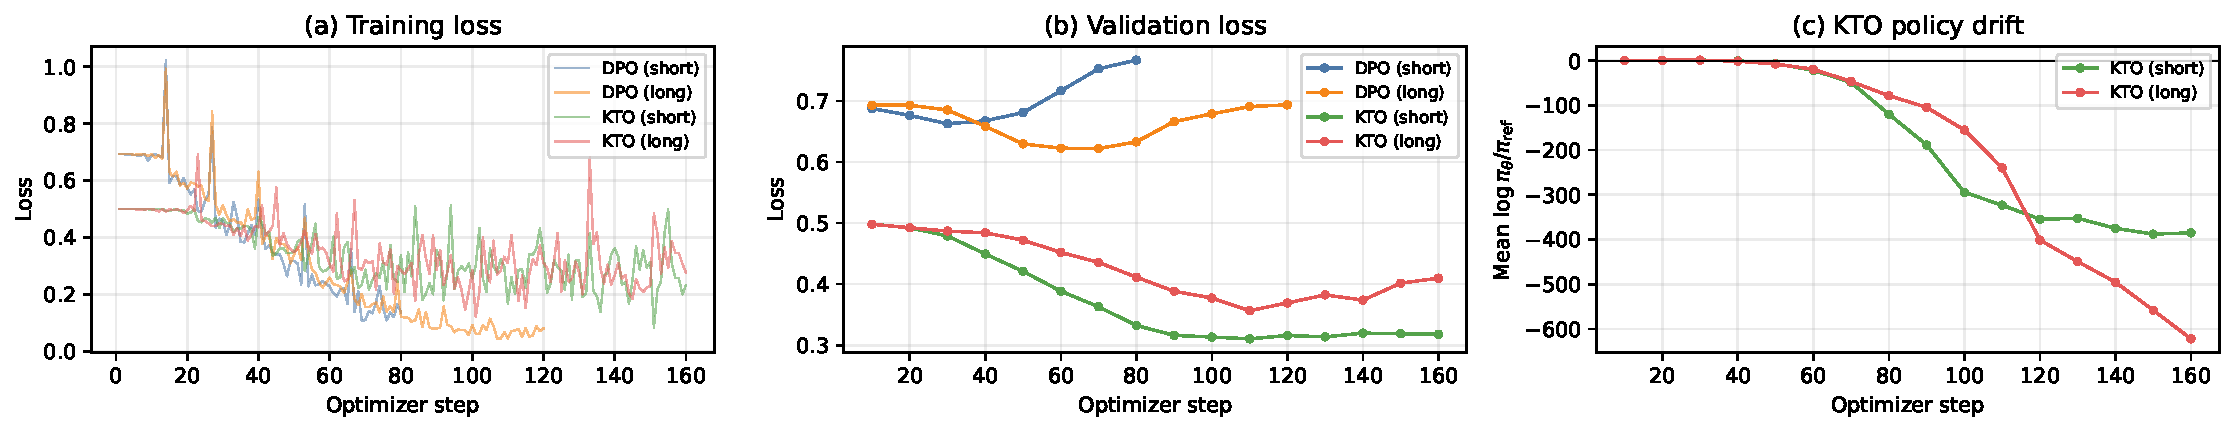
\includegraphics[width=\linewidth]{figures/training_curves.pdf}
\caption{Training diagnostics: (a) training loss, (b) validation loss, (c) KTO validation log-ratio $\mathbb{E}[\log \pi_\theta / \pi_\text{ref}]$.  KTO's log-ratio collapse (panel c) is discussed in \S\ref{sec:ktodrift}.}
\label{fig:training}
\end{figure*}

\begin{figure*}[!t]
\centering
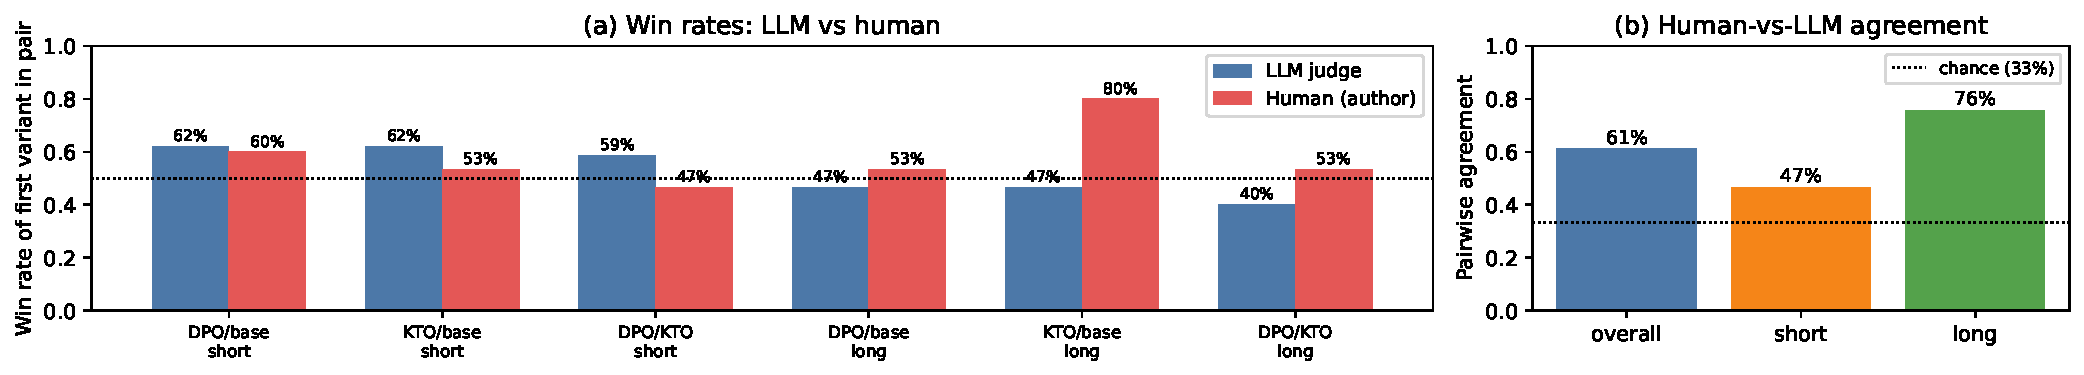
\includegraphics[width=\linewidth]{figures/agreement_matrix.pdf}
\caption{LLM vs human win rates per comparison (left) and pairwise agreement breakdown (right).}
\label{fig:agree}
\end{figure*}

\subsection{Data and splits}
The 502 prompts are split 30 / 472, with 30 held out for evaluation and the remaining 472 split 90/10 into train and val.  Class balance on the KTO binary task is uneven (37\% desirable, 59\% undesirable in the short condition), which makes KTO's inverse-frequency weighting load-bearing rather than cosmetic.

\subsection{Training dynamics}
Best-val-loss checkpoint selection (Figure~\ref{fig:training}a,b) picks step~30 for DPO short, 70 for DPO long, and 110 for both KTO variants.  DPO overfits visibly in the second half (train collapses, val rises); KTO long bottoms then degrades.

\subsection{Cross-judge results}
The dominant pattern in the cross-judge rankings is a context-length effect: short-context fine-tuning improves both algorithms over the base model (DPO 62\%, KTO 62\%), while long-context fine-tuning \emph{degrades} both below base (DPO 47\%, KTO 47\%).  Head-to-head, DPO beats KTO on short (59--41) while KTO beats DPO on long (60--40), suggesting algorithm choice should be made jointly with context length rather than independently.  Table~\ref{tab:quant} consolidates these numbers alongside the validation losses and reveals a disagreement: KTO achieves lower val loss than DPO in both context conditions (0.310 vs 0.663 short; 0.357 vs 0.622 long), yet the cross-judge ranks the two in the \emph{opposite} order on the short condition.  The mechanism is in \S\ref{sec:ktodrift}.

\begin{table}[!htb]
\centering
\small
\setlength{\tabcolsep}{6pt}
\begin{tabular}{lccc}
\toprule
Variant & Val loss $\downarrow$ & WR vs base $\uparrow$ & Perp.\ $\downarrow$ \\
\midrule
Base short              & ---    & ---  & 3.25 \\
DPO short    & 0.663  & 0.62 & 2.68 \\
KTO short    & 0.310  & 0.62 & 2.97 \\
\midrule
Base long               & ---    & ---  & 2.88 \\
DPO long    & 0.622  & 0.47 & 3.02 \\
KTO long    & 0.357  & 0.47 & 2.95 \\
\bottomrule
\end{tabular}
\caption{Quantitative results.  Win rate is against base on the matching context; perplexity is under the frozen base model.}
\label{tab:quant}
\end{table}

\subsection{KTO's validation loss masks policy drift}
\label{sec:ktodrift}
KTO's loss has an upper bound: once the policy is confidently wrong enough, the loss saturates near its cap and stops giving the optimizer useful gradient, but nothing in the loss prevents the policy from drifting further from the reference.  Figure~\ref{fig:training}(c) shows this happening: validation loss falls monotonically while the mean validation log-ratio $r_\theta = \log\pi_\theta - \log\pi_\text{ref}$ crashes to $\sim-400$ (KTO short) and below $-600$ (KTO long).  At those values the trained policy is assigning the average eval response a probability $\sim e^{-400}$ times the reference, which is effectively a different model and is consistent with KTO long's 47\% cross-judge win rate against base.  DPO does not collapse this way because its loss is unbounded; if the margin goes the wrong way, $-\log\sigma$ blows up and the optimizer is forced to fight drift.

Pal et al.\ \cite{pal2024smaug} reported a related issue in DPO where the chosen-response probability can drop below the reference, and patched it with an added regularizer (DPO-Positive).  We see KTO's analog as not needing a regularizer at all: the policy-vs-reference log-ratio is already directly observable during training, and gating on it rather than on validation loss is enough to catch this failure mode.

\paragraph{Human validation.}
\label{sec:humanval}
Figure~\ref{fig:agree} compares the two judges.  Pairwise agreement (protocol in \S\ref{sec:method}) is 61\% overall (Cohen's $\kappa = 0.34$ on the top pick), asymmetric by context: long 76\%, short 47\% (short-context distinctions are subtle).  The biggest disagreement is KTO long vs base, where humans pick KTO long 80\% of the time but the LLM only 47\%.

\paragraph{Qualitative.}
On a one-liner prompt about British Airways' £1.7bn fuel hit and the Iran war:

\noindent\textbf{Base.}  ``Why don't British Airways fly Boeing 747s anymore? Because those fuel bills are so high, they'd need to charge a premium BA fare just to fill up the jumbo jets.''  (Generic; the article isn't really doing any work.)

\noindent\textbf{DPO short.}  ``Why did British Airways increase their prices like a hot air balloon? To recover the €2bn fuel bill from the Iran-Iraq price war.''  (Pulls in the actual numbers and the geopolitical hook.)

\noindent\textbf{KTO short.}  ``Why did British Airways hike up their premium fares? To cover the £1.7bn unexpected fuel bill they incurred after buying tickets to Iran's war of words and lost their fuel hedging bet?''  (Article-specific and includes a finance term, but punchline meanders.)

On the same prompt in long context, the base model emits the literal tag \verb|<alternate_jokes>| inside its response, a representative prompt-template leakage discussed in the limitations.
